\chapter{Introduction}

When we try to research on the topic about cryptography, a natural question is: how can we tell whether a cryptographic construction is “really secure” against real-world attackers? Broadly speaking there are two routes. One is destructive—designing algorithms and make experiments to find attacks and counterexamples. The other is constructive—providing security proofs that can be independently reproduced and proved. This paper follows the constructive approach and goes a step further by mechanizing the proofs: we translate security into executable games and reductions, and use a proof assistant to automatically check each step of the reasoning.

In particular, we study a classical ElGamal Key Encapsulation Mechanism (\KEM) and its security in the attack model that allows decryption queries before the challenge is issued, denoted \INDCCAone. At the same time we consider a algebraic hardness assumption, the q-Decisional Diffie–Hellman problem (\qDDH). Our central claim is that, under accurate and suitable formalisation, breaking the \INDCCAone security of the ElGamal \KEM is essentially the same task as distinguishing the two distributions in the \qDDH problem for the same parameters. In other words, the two problems are equivalent and tight: given any adversary on one side we can covert it without loss to an adversary on the other side, preserving the adversary’s success probability up to negligible loss.

Intuitively, \INDCCAone allows the adversary to query a decryption oracle a limited number of times before receiving a single challenge ciphertext, but still requires that the adversary cannot distinguish a real session key from a random key. The \qDDH problem asks that, even if an adversary obtains several group elements corresponding to powers of a secret exponent, it cannot distinguish whether a given element corresponds to a true Diffie–Hellman product or to random generated. In the algebraic group setting, we want to trace adversarial group elements through their linear relations to known generators, which allows for constructing verifiable oracle responses. This technique enable us tightly mechanized correspondence between the two security frameworks.


\section{Motivation}



Public-key cryptography forms the foundation of modern secure cryptographic systems, enabling the confidential exchange of information over untrusted networks. Among its fundamental security notions, Key Encapsulation Mechanisms (\KEM) play a crucial role in constructing shared symmetric keys for subsequent encrypted communication\cite{Sharifian2021}. 
To remain secure against active attackers, these mechanisms require strong security guarantees, with indistinguishability under chosen-ciphertext attacks (IND-CCA) being among the most demanding and practically relevant.
The \INDCCAone variant, where adversaries have access to a decryption oracle only before seeing the challenge ciphertext, reflects many real-world attack scenarios while remaining trackable for theoretical analysis.



The ElGamal-based KEM, derived from the classical ElGamal construction, bases its security on the discrete logarithm problem in cyclic groups\cite{Sven2024}.

While ElGamal in its original public-key encryption form achieves only IND-CPA security~\cite{pandey2021}, its KEM formulation enables stronger guarantees when analyzed under appropriate computational assumptions\cite{Sven2024}. 
However, providing a fully formal and tight IND-CCA1 proof in the standard model remains challenging, often requiring non-trivial or idealized assumptions.

The Algebraic Group Model (AGM), introduced by Fuchsbauer, Kiltz, and Loss\cite{fuchsbauer2018}, provides a middle ground between the standard model and idealized models such as the random oracle model. 
In the AGM, adversaries are restricted to be \emph{algebraic}, meaning they can only produce group elements for which they can provide explicit representations in terms of previously seen group elements. This restriction represents the intuition that adversaries cannot produce group elements arbitrarily but must construct them through the algebraic structure of existing elements.

The AGM has proven particularly valuable for analyzing the security of cryptographic schemes based on discrete logarithm assumptions. It enables proofs that would be infeasible in the standard model while avoiding the oversimplifications of purely idealized settings\cite{Bauer2021}. Recent work has highlights that many schemes, including digital signatures~\cite{fersch2018} and KEMs derived from ElGamal, can be proven secure under standard hardness assumptions when analyzed in the AGM.



Our work builds on this foundation by leveraging AGM-style techniques to indicates the IND-CCA1 security of ElGamal-based \KEM under the \qDDH assumption. Although our proof does not require the full AGM framework, it employs the key insight that adversaries' group-element productions can be tracked through linear algebraic representations, enabling sophisticated oracle simulation techniques.

In addition, the mechanized proof formalizes a bilateral reduction between the \INDCCAone security of the ElGamal-based \KEM and the \qDDH assumption in EasyCrypt, establishing a computational equivalence that ensures the proof’s tightness and soundness.

The proofs are mechanized in the EasyCrypt proof assistant\cite{easycrypt}, which is tailored for game-based cryptographic proofs at code level and gives support for common proof techniques, for instance, byequiv transformations, probabilistic reasoning, random variable transformations and algebraic manipulation techniques, it has been widely applied to build the security of the majority of cryptographic primitives and to connect with formalized proofs and their particular implementations.

Our main theorem can be informally phrased as follows:
\begin{quote}
\emph{The ElGamal-based Key Encapsulation Mechanism (\KEM) is \INDCCAone secure under the q-DDH assumption in cyclic groups of prime order and adversaries are modeled as algebraic in the sense of the AGM\cite{fuchsbauer2018}.}
\emph{The reduction between an IND-CCA1 adversary against ElGamal-based \KEM and a distinguisher for the q-DDh problem is tight, ensuring equality of advantages up to negligible terms. The security bound holds unconditionally with respect to the simulation, without loss beyond polynomial overhead. }
\end{quote}






\section{Problem Statement}

The central question we address is:

\begin{quote}
\emph{Can we introduce a formal and bidirectional methodology, with tight concrete bounds, the equivalence between breaking IND-CCA1 security of ElGamal-based \KEM and solving the q-DDH problem, with both  reductions mechanized and machine-checked?}
\end{quote}

This research question requires several non-trivial technical challenges that required to be carefully addressed in order to build a mechanized proof

\begin{enumerate}
\item \textbf{Reduction Construction}: The core of our work is to design precise and efficient reductions that bridge the IND-CCA1 security game with the q-DDH problem. Precisely, the reduction is required to translate any IND-CCA1 adversary against ElGamal-based \KEM into a distinguisher for q-DDH, and conversely, it should also established an methodology to transform a q-DDH distinguisher into IND-CCA1 adversary. Achieving this requires a careful embedding of the q-DDH challenge into the Elgamal-based \KEM experiment while preserving the advantage of adversary. 
In conclusion, the challenge is not only in defining the reduction accurately but also in ensuring that it do not tolerate any loss of advantage occurs.

\item \textbf{Oracle Simulation}: One of the most delicate and significant aspects of our security proofs is the establishment of a decryption oracle simulator. This orcale is required to be consistently answering adversarial queries while withholding information that would trivialize the underlying hard problems. In our setting, this needs simulating decryption queries in a way that is consistent with the \qDDH challenge without revealing the hidden exponent. This is particularly challenging under the AGM, where adversaries provide linear representations of ciphertexts. The simulator is required to make leverage of these representations to provide faithful reflections while not leaking unintended information.
\item \textbf{Formal Verification}: Despite the high-level construction, our objective is to formalize and mechanize the entire reduction within the EasyCrypt, which requires us to encode all probabilistic reasoning, hybrid argument and algebraic manipulation in order to checked by the machine. In contrast to traditional paper proofs, where intuition often fills in the gaps. Constraints on length, representation validity and randomness-preserving transformations must all be explicitly formalized. In conclusion the key challenge is reconciling the intuitive reasoning of algebraic reductions with the strict requirements of mechanized verification framework.

\item \textbf{Tightness Analysis}: Finally, it is essential to illustrate the reduction is not only accurate but also tight in a concrete security sense. It involves proving that the adversarial is maintained exactly when transforming between the IND-CCA1 and q-DDH games. Constructing such concrete bounds is significant for the practical relevance of our results, while it ensures that the hardness of the q-DDH problem directly translates to the security guarantees for ElGamal-based \KEM. Additionally, by examining tightness, it enables us to gain insight into the efficiency of the reductions and be able to verify that the proof has avoided artificial losses of security that might otherwise reduce its practical impact.
\end{enumerate}

% \begin{figure}[htbp]
% \centering
% \begin{tikzpicture}[
%     node distance=3cm,
%     game/.style={rectangle, draw, fill=blue!15, text width=5.5cm, text centered, minimum height=3.5cm, rounded corners=4pt},
%     scheme/.style={rectangle, draw, fill=green!15, text width=4.5cm, text centered, minimum height=2.8cm, rounded corners=4pt},
%     reduction/.style={rectangle, draw, fill=orange!15, text width=4cm, text centered, minimum height=2cm, rounded corners=4pt},
%     arrow/.style={->, thick, >=stealth},
%     equiv/.style={<->, very thick, blue, >=stealth}
% ]

% % IND-CCA1 Game
% \node[game] (indcca-game) at (-10.5,5) {
%     \textbf{IND-CCA1 Game}\\[0.3cm]
%     \footnotesize
%      $(pk, sk) \leftarrow \text{Gen}()$\\
%      $b' \leftarrow A^{\text{Dec},\text{Enc}}(pk)$\\
%      Return $b'$\\[0.3cm]
%     \textbf{Dec}$(C)$ // Before Enc\\
%      $K \leftarrow \text{Dec}(C, sk)$\\
%      Return $K$\\[0.3cm]
%     \textbf{Enc}$()$ // One time\\
%      $(K_0^*, C^*) \leftarrow \text{Enc}(pk)$\\
%      $K_1^* \leftarrow \mathcal{K}$\\
%      Return $(K_b^*, C^*)$
% };

% % q-DDH Game  
% \node[game] (qddh-game) at (0.5,5) {
%     \textbf{q-DDH Game}\\[0.3cm]
%     \footnotesize
%      $x, r, z \leftarrow \mathbb{Z}_p$\\
%      $b' \leftarrow A(g^x, g^{x^2}, \ldots, g^{x^q},$\\
%     \phantom{01 $b' \leftarrow A($}$g^r, g^{xr+zb})$\\
%      Return $b'$
% };

% % ElGamal Scheme
% \node[scheme] (elgamal) at (-10.5,-8) {
%     \textbf{ElGamal KEM}\\[0.3cm]
%     \footnotesize
%     \textbf{Gen}$(\mathcal{G})$:\\
%      $x \leftarrow \mathbb{Z}_p$\\
%      $X := g^x$\\
%     Return $(pk, sk) := (X, x)$\\[0.3cm]
%     \textbf{Enc}$(pk)$:\\
%      $r \leftarrow \mathbb{Z}_p$\\
%     $C := g^r$\\
%      $K := X^r$\\
%      Return $(K, C)$\\[0.3cm]
%     \textbf{Dec}$(C, sk)$:\\
%      If $C \notin \mathcal{G}$ Return $\perp$\\
%      $K := C^x$\\
%      Return $K$
% };

% % q-DDH Problem Structure
% \node[scheme] (qddh-structure) at (0.5,-6) {
%     \textbf{q-DDH Structure}\\[0.3cm]
%     \footnotesize
%     Given: $(g^x, g^{x^2}, \ldots, g^{x^q}, g^r, T)$\\[0.3cm]
%     Distinguish:\\
%     • $T = g^{xr}$ (real)\\
%     • $T = g^{xr+z}$ (random)\\[0.3cm]
%     where $x, r, z \leftarrow \mathbb{Z}_p$
% };
% % Forward Reduction
% \node[reduction] (forward-red) at (-7.5,-0.5) {
%     \textbf{${\text{A\_from\_INDCCA1}}(B)$}\\[0.2cm]
%     \footnotesize
%     • Receives q-DDH challenge\\
%     • Sets $pk = g^x$\\
%     • Simulates limited Dec oracle\\
%     • Uses linear representations\\
%     • Outputs q-DDH decision
% };

% % Backward Reduction
% \node[reduction] (backward-red) at (-2.5,0.5) {
%     \textbf{${\text{B\_from\_qDDH}}(A)$}\\[0.2cm]
%     \footnotesize
%     • Embeds q-DDH challenge\\
%     • Simulates IND-CCA1 game\\
%     • Programs challenge ciphertext\\
%     • Uses same oracle discipline\\
%     • Outputs IND-CCA1 guess
% };
% % Main equivalence
% \draw[equiv] (indcca-game) -- (qddh-game) node[midway, above] {\textbf{Tight Bilateral Equivalence}};

% % Connections to schemes
% \draw[arrow] (indcca-game) -- (elgamal) node[midway, left] {uses};
% \draw[arrow] (qddh-game) -- (qddh-structure) node[midway, right] {based on};

% % Reduction arrows
% \draw[arrow] (elgamal) -- (forward-red) node[midway, below left, sloped] {input};
% \draw[arrow] (forward-red) -- (qddh-structure) node[midway, below right, sloped] {output};

% \draw[arrow] (qddh-structure) -- (backward-red) node[midway, below right, sloped] {input};
% \draw[arrow] (backward-red) -- (elgamal) node[midway, below left, sloped] {output};

% % Oracle simulation details
% \node[draw, fill=yellow!10, text width=8cm, rounded corners] (oracle-details) at (-3.75,-10) {
%     \textbf{Key Technical Components:}\\[0.2cm]
%     • Limited Decryption Oracle: requires $c = \text{prodEx}(l, z)$\\
%     • Linear Algebra Library: \texttt{prodEx}, \texttt{addv}, \texttt{scalev}, \texttt{sumv}\\
%     • 30+ Supporting Lemmas: distributivity, scaling, base reduction\\
%     • Tight Analysis: $\mathsf{Adv}_{\text{IND-CCA1}} = \mathsf{Adv}_{\text{q-DDH}}$
% };

% \draw[arrow, dotted] (forward-red) -- (oracle-details);
% \draw[arrow, dotted] (backward-red) -- (oracle-details);

% \end{tikzpicture}
% \caption{Detailed bilateral reduction between IND-CCA1 security of ElGamal-based \KEM and \qDDH hardness, showing the complete game structures and algorithmic details.}
% \label{fig:detailed-bilateral-reduction}
% \end{figure}

\newpage

\section{Main Contributions}

Our work makes several significant contributions to both theoretical cryptography and formal verification:

\begin{enumerate}
\item \textbf{Reduction Theorem}: We prove the \texttt{qDDH\_Implies\_INDCCA1\_ElGamal }and \newline \texttt{INDCCA1\_ElGamal\_Implies\_qDDH} lemma, establishing the equivalence between q-DDH hardness and IND-CCA1 security:
  \[
  \Pr[\text{IND\_CCA1\_P}(\text{ElGamal}, B).\text{main}() : \text{res}] = \Pr[\text{QDDH}(A_{\text{from\_INDCCA1}}(B)).\text{main}() : \text{res}]
  \]

\item \textbf{Oracle Simulation Technique}: We develop a sophisticated method for simulating the decryption oracle which utilizes linear algebraic representations to remain consistency without circular dependencies.

\item \textbf{Linear Algebra Library}: We contribute a reusable library of operators and their lemmas to EasyCrypt codebase that able to solve linear algebraic operations over exponents:
  \begin{itemize}
  \item Core operators: \texttt{prodEx}, \texttt{addv}, \texttt{scalev}, \texttt{sumv}, \texttt{shift\_trunc}
  \item Over 30  lemmas of distributivity, scaling, base reduction, and vector operations
  \item Reusable components for AGM proofs with linear combinations
  \end{itemize}

\item \textbf{Complete EasyCrypt Formalization}: Our proof is entirely mechanized using EasyCrypt, comprising over 2000 lines code, with extensive documentation and modular design for future usage.

\item \textbf{Tight Security Analysis}: We indicate that our reduction is tight, without security loss, providing optimal concrete security bounds.
\end{enumerate}







\newpage


\begin{figure}[H]
\centering
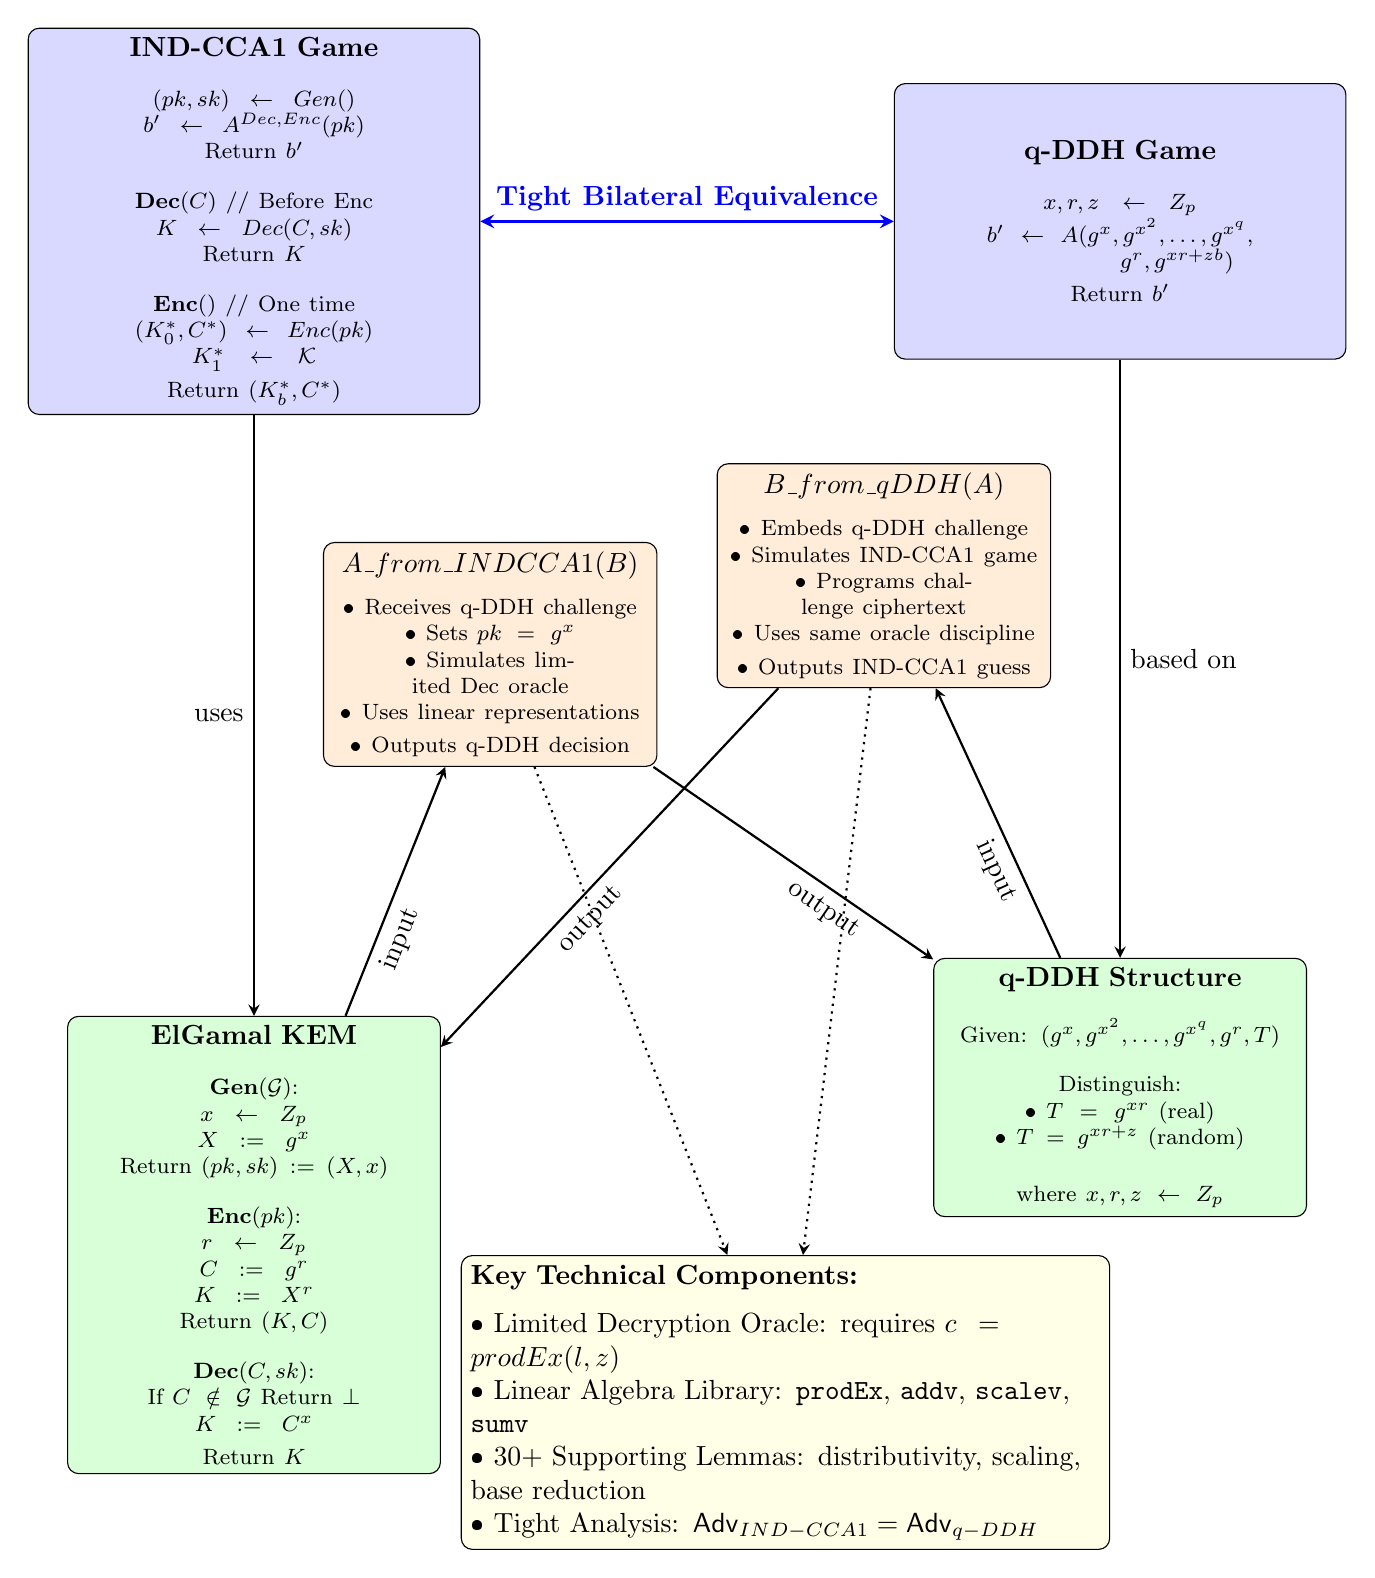
\begin{tikzpicture}[
    node distance=3cm,
    game/.style={rectangle, draw, fill=blue!15, text width=5.5cm, text centered, minimum height=3.5cm, rounded corners=4pt},
    scheme/.style={rectangle, draw, fill=green!15, text width=4.5cm, text centered, minimum height=2.8cm, rounded corners=4pt},
    reduction/.style={rectangle, draw, fill=orange!15, text width=4cm, text centered, minimum height=2cm, rounded corners=4pt},
    arrow/.style={->, thick, >=stealth},
    equiv/.style={<->, very thick, blue, >=stealth}
]

% IND-CCA1 Game
\node[game] (indcca-game) at (-10.5,5) {
    \textbf{IND-CCA1 Game}\\[0.3cm]
    \footnotesize
     $(pk, sk) \leftarrow \text{Gen}()$\\
     $b' \leftarrow A^{\text{Dec},\text{Enc}}(pk)$\\
     Return $b'$\\[0.3cm]
    \textbf{Dec}$(C)$ // Before Enc\\
     $K \leftarrow \text{Dec}(C, sk)$\\
     Return $K$\\[0.3cm]
    \textbf{Enc}$()$ // One time\\
     $(K_0^*, C^*) \leftarrow \text{Enc}(pk)$\\
     $K_1^* \leftarrow \mathcal{K}$\\
     Return $(K_b^*, C^*)$
};

% q-DDH Game  
\node[game] (qddh-game) at (0.5,5) {
    \textbf{q-DDH Game}\\[0.3cm]
    \footnotesize
     $x, r, z \leftarrow \mathbb{Z}_p$\\
     $b' \leftarrow A(g^x, g^{x^2}, \ldots, g^{x^q},$\\
    \phantom{01 $b' \leftarrow A($}$g^r, g^{xr+zb})$\\
     Return $b'$
};

% ElGamal Scheme
\node[scheme] (elgamal) at (-10.5,-8) {
    \textbf{ElGamal KEM}\\[0.3cm]
    \footnotesize
    \textbf{Gen}$(\mathcal{G})$:\\
     $x \leftarrow \mathbb{Z}_p$\\
     $X := g^x$\\
    Return $(pk, sk) := (X, x)$\\[0.3cm]
    \textbf{Enc}$(pk)$:\\
     $r \leftarrow \mathbb{Z}_p$\\
    $C := g^r$\\
     $K := X^r$\\
     Return $(K, C)$\\[0.3cm]
    \textbf{Dec}$(C, sk)$:\\
     If $C \notin \mathcal{G}$ Return $\perp$\\
     $K := C^x$\\
     Return $K$
};

% q-DDH Problem Structure
\node[scheme] (qddh-structure) at (0.5,-6) {
    \textbf{q-DDH Structure}\\[0.3cm]
    \footnotesize
    Given: $(g^x, g^{x^2}, \ldots, g^{x^q}, g^r, T)$\\[0.3cm]
    Distinguish:\\
    • $T = g^{xr}$ (real)\\
    • $T = g^{xr+z}$ (random)\\[0.3cm]
    where $x, r, z \leftarrow \mathbb{Z}_p$
};
% Forward Reduction
\node[reduction] (forward-red) at (-7.5,-0.5) {
    \textbf{${\text{A\_from\_INDCCA1}}(B)$}\\[0.2cm]
    \footnotesize
    • Receives q-DDH challenge\\
    • Sets $pk = g^x$\\
    • Simulates limited Dec oracle\\
    • Uses linear representations\\
    • Outputs q-DDH decision
};

% Backward Reduction
\node[reduction] (backward-red) at (-2.5,0.5) {
    \textbf{${\text{B\_from\_qDDH}}(A)$}\\[0.2cm]
    \footnotesize
    • Embeds q-DDH challenge\\
    • Simulates IND-CCA1 game\\
    • Programs challenge ciphertext\\
    • Uses same oracle discipline\\
    • Outputs IND-CCA1 guess
};
% Main equivalence
\draw[equiv] (indcca-game) -- (qddh-game) node[midway, above] {\textbf{Tight Bilateral Equivalence}};

% Connections to schemes
\draw[arrow] (indcca-game) -- (elgamal) node[midway, left] {uses};
\draw[arrow] (qddh-game) -- (qddh-structure) node[midway, right] {based on};

% Reduction arrows
\draw[arrow] (elgamal) -- (forward-red) node[midway, below left, sloped] {input};
\draw[arrow] (forward-red) -- (qddh-structure) node[midway, below right, sloped] {output};

\draw[arrow] (qddh-structure) -- (backward-red) node[midway, below right, sloped] {input};
\draw[arrow] (backward-red) -- (elgamal) node[midway, below left, sloped] {output};

% Oracle simulation details
\node[draw, fill=yellow!10, text width=8cm, rounded corners] (oracle-details) at (-3.75,-10) {
    \textbf{Key Technical Components:}\\[0.2cm]
    • Limited Decryption Oracle: requires $c = \text{prodEx}(l, z)$\\
    • Linear Algebra Library: \texttt{prodEx}, \texttt{addv}, \texttt{scalev}, \texttt{sumv}\\
    • 30+ Supporting Lemmas: distributivity, scaling, base reduction\\
    • Tight Analysis: $\mathsf{Adv}_{\text{IND-CCA1}} = \mathsf{Adv}_{\text{q-DDH}}$
};

\draw[arrow, dotted] (forward-red) -- (oracle-details);
\draw[arrow, dotted] (backward-red) -- (oracle-details);

\end{tikzpicture}
\caption{Detailed bilateral reduction between IND-CCA1 security of ElGamal-based \KEM and \qDDH hardness, showing the complete game structures and algorithmic details.}
\label{fig:detailed-bilateral-reduction}
\end{figure}




\section{Technical Overview}

Figure~\ref{fig:detailed-bilateral-reduction} indicates an intuitive overview of our proof technique.
At a high level, our goal is to show that the capability to break the IND-CCA1 security of the ElGamal-based \KEM\ is computationally equivalent to handling the \qDDH\ problem. 
Instead of relying on a one-way reduction, our analysis establishes a \emph{two-direction correspondence}—showing that both can be transformed into the other without any meaningful loss.

The proof process by building two designed reductions. 
In the \textbf{first direction}, we indicate that any adversary ability to breaking the ElGamal \KEM\ under chosen-ciphertext attacks can be covert into an algorithm that handle the \qDDH\ challenge. 
In the \textbf{reverse direction}, we demonstrate that a successful \qDDH\ distinguisher can be used to build an adversary that breaks the \KEM.

A key technical component is the leverage of \textbf{algebraic tracking}, where every group element generated during the simulation is represented as a linear combination of previously known ones. 
This idea, inspired by the Algebraic Group Model~\cite{cong2022}, ensures that simulated oracles behave consistently and ensures every adversarial action has a verifiable algebraic explanation.

Finally, the entire framework, containing oracle simulations, linear algebra operators (\texttt{prodEx}, \texttt{addv}, \texttt{scalev}, and \texttt{sumv}), and supporting lemmas—is implemented and mechanically verified in the \textsc{EasyCrypt} proof assistant, which guarantees the correspondence between the two games is not only theoretically sound but also \emph{machine-checked}.


% \subsection{Problem Structure and Games}

% The foundation of proof lies in the characterization of two computation problems:

% \subsubsection{IND-CCA1 Security Game.} 

% The indistinguishability under chosen-ciphertext attacks (IND-CCA1) security game for ElGamal \KEM proceeds as follows: The challenger first introduce a key pair $\text{Gen}()\rightarrow(pk,sk)$ where $pk = g^x$ and $sk = x$ for a randomly chosen $x \leftarrow \mathbb{Z}_p$. Then, the adversary $A$ is given the public key $pk$ and then make decryption queries to a oracle $\text{Dec}(C, sk)$ that returns $K = C^x$ for valid ciphertexts $C \in \mathcal{G}$. At some point, the adversary requests a challenge by calling the encryption oracle only once. The challenger computes $ \text{Enc}(pk)\rightarrow(K_0^*, C^*)$ where $C^* = g^r$ and $K_0^* = (g^x)^r = g^{xr}$ for a  random $ \mathbb{Z}_p \rightarrow r$, then selects a random key $ \mathcal{K} \rightarrow K_1^*$, and finally return $(K_b^*, C^*)$ for a random bit $b$. Finally, The adversary will outputs a guess $b'$ and wins if $b' = b$.

% The algorithm specification\cite{fuchsbauer2018} is detailed in Figure~\ref{fig:indcca1-algorithm}.

% \begin{figure}[H]
% \centering
% \footnotesize
% \begin{tabular}{|p{15cm}|}
% \hline
% \multicolumn{1}{|c|}{\textbf{IND-CCA1$_{\text{EG},\mathcal{G}}^A$ Security Game for ElGamal}} \\
% \hline
% \textbf{Algorithm:} \\
% 00 $x \leftarrow \mathbb{Z}_p$ \\
% 01 $X := g^x$ \\
% 02 $b' \leftarrow A^{\text{Dec},\text{Enc}}(X)$ \\
% 03 Return $b'$ \\
% \hline
% \textbf{Oracles Available to Adversary } $A$\textbf{:} \\
% $\bullet$ \textbf{Dec}$(C)_a$ // Before Enc is called \\
% \phantom{$\bullet$} 04 If $C \notin \mathcal{G}$ Return $\perp$ \\
% \phantom{$\bullet$} 05 $K := C^x$ \\
% \phantom{$\bullet$} 06 Return $K$ \\
% \\
% $\bullet$ \textbf{Enc}$()$ // One time only \\
% \phantom{$\bullet$} 07 $r \leftarrow \mathbb{Z}_p$ \\
% \phantom{$\bullet$} 08 $C^* := g^r$ \\
% \phantom{$\bullet$} 09 $K^* := X^r$ \\
% \phantom{$\bullet$} 10 $K_1^* \leftarrow \mathcal{K}$ // random key \\
% \phantom{$\bullet$} 11 $b \leftarrow \{0,1\}$ \\
% \phantom{$\bullet$} 12 Return $(K_b^*, C^*)$ \\
% \hline
% \textbf{ElGamal KEM Operations:} \\
% $\bullet$ \textbf{Gen}$(\mathcal{G}) \rightarrow (pk, sk)$: $x \leftarrow \mathbb{Z}_p$; $X := g^x$; Return $(X, x)$ \\
% $\bullet$ \textbf{Enc}$(pk) \rightarrow (K, C)$: $r \leftarrow \mathbb{Z}_p$; $C := g^r$; $K := pk^r$; Return $(K, C)$ \\
% $\bullet$ \textbf{Dec}$(C, sk) \rightarrow K$: If $C \notin \mathcal{G}$ Return $\perp$; $K := C^{sk}$; Return $K$ \\
% \hline
% \textbf{Advantage Definition:} \\
% $\mathsf{Adv}^{\text{IND-CCA1}}_{\text{ElGamal}}(A) = \left|\Pr[b' = b] - \frac{1}{2}\right|$ \\
% where $b$ is the random bit used in the Enc oracle \\
% \hline
% \textbf{Security Goal:} \\
% Adversary $A$ should not be able to distinguish between $K_0^* = g^{xr}$ (real key) and $K_1^*$ (random key) \\
% even with access to decryption oracle before receiving the challenge $(K_b^*, C^*)$ \\
% \hline
% \end{tabular}
% \caption{IND-CCA1 security game for ElGamal encryption. The adversary has access to a decryption oracle before the challenge phase, then must distinguish between a real session key and a random key.}
% \label{fig:indcca1-algorithm}
% \end{figure}






% \subsubsection{q-DDH Problem.} The q-Decisional Diffie-Hellman (q-DDH) problem will ask one to distinguish between two distributions over group elements. 
% By given a tuple $(g^x, g^{x^2}, \ldots, g^{x^q}, g^r, T)$ where $x, r \leftarrow \mathbb{Z}_p$ are random, the attacker must determine whether $T = g^{xr}$ (real distribution) or $T = g^{xr+z}$ for a random $z \leftarrow \mathbb{Z}_p$ (random distribution).

% The specification\cite{fuchsbauer2018} is detailed below in Figure~\ref{fig:qddh-algorithm}.


% \begin{figure}[H]
% \centering
% \footnotesize
% \begin{tabular}{|p{15cm}|}
% \hline
% \multicolumn{1}{|c|}{\textbf{q-DDH$_{\mathcal{G},q}^A$ Problem}} \\
% \hline
% \textbf{Algorithm:} \\
% 00 $x, r, z \leftarrow \mathbb{Z}_p$ \\
% 01 $b \leftarrow \{0,1\}$ \\
% 02 $T_0 := g^{xr}$, $T_1 := g^{xr+z}$ \\
% 03 $b' \leftarrow A(g^x, g^{x^2}, \ldots, g^{x^q}, g^r, T_b)$ \\
% 04 Return $b'$ \\
% \hline
% \textbf{Challenge Structure Given to Distinguisher } $A$\textbf{:} \\
% $\bullet$ \textbf{Powers of } $x$: $(g^x, g^{x^2}, g^{x^3}, \ldots, g^{x^q})$ \\
% $\bullet$ \textbf{Random element:} $g^r$ where $r \leftarrow \mathbb{Z}_p$ \\
% $\bullet$ \textbf{Target element:} $T \in \{g^{xr}, g^{xr+z}\}$ where $z \leftarrow \mathbb{Z}_p$ \\
% \hline
% \textbf{Distinguishing Goal:} \\
% $\bullet$ \textbf{Real distribution } $\mathcal{D}_0$: $T = g^{xr}$ (DDH tuple) \\
% $\bullet$ \textbf{Random distribution } $\mathcal{D}_1$: $T = g^{xr+z}$ (random element) \\
% \\
% Distinguisher $A$ must output a bit $b'$ indicating which distribution the challenge comes from \\
% \hline
% \textbf{Advantage Definition:} \\
% $\mathsf{Adv}^{q\text{-DDH}}_{\mathcal{G}}(A) = \left|\Pr[A(\mathcal{D}_0) = 1] - \Pr[A(\mathcal{D}_1) = 1]\right|$ \\
% where $\mathcal{D}_0 = (g^x, g^{x^2}, \ldots, g^{x^q}, g^r, g^{xr})$ \\
% and $\mathcal{D}_1 = (g^x, g^{x^2}, \ldots, g^{x^q}, g^r, g^{xr+z})$ \\
% \hline
% \textbf{Hardness Assumption:} \\
% For any probabilistic polynomial-time algorithm $A$: \\
% $\mathsf{Adv}^{q\text{-DDH}}_{\mathcal{G}}(A) \leq \text{negl}(\lambda)$ \\
% \\
% The q-DDH assumption states that even given the first $q$ powers of $x$, \\
% it remains computationally hard to distinguish $g^{xr}$ from $g^{xr+z}$ \\
% \hline
% \textbf{Relationship to Standard DDH:} \\
% $\bullet$ Standard DDH: Given $(g^a, g^b, g^c)$, distinguish $c = ab$ from random $c$ \\
% $\bullet$ q-DDH: Given $(g^x, \ldots, g^{x^q}, g^r, T)$, distinguish $T = g^{xr}$ from $T = g^{xr+z}$ \\
% $\bullet$ q-DDH $\Rightarrow$ DDH but the converse may not hold \\
% \hline
% \end{tabular}
% \caption{q-DDH (q-Decisional Diffie-Hellman) problem. The distinguisher receives the first $q$ powers of a secret exponent $x$ along with $g^r$ and must distinguish between $g^{xr}$ and $g^{xr+z}$ for random $z$.}
% \label{fig:qddh-algorithm}
% \end{figure}
















% \subsection{Bilateral Reduction Strategy}

% Our core technical contribution is the establishment of two reductions that bridge computational equivalence between:

% \subsubsection{Forward Reduction: ${\text{A\_from\_INDCCA1}}$.} This reduction will convert all IND-CCA1 adversary $B$ against ElGamal into a q-DDH distinguisher.,which works as follows:
% \begin{enumerate}
% \item \textbf{Challenge Reception:} It will first receiving a q-DDH challenge $(g^x, g^{x^2}, \ldots, g^{x^q}, g^r, T)$, then set the public key as $pk = g^x$.
% \item \textbf{Oracle Simulation:} Then it will leverage a limited decryption oracle that only processes queries $(C, z)$ where  adversary provides an explicit linear representation $z$ such that $C = \text{prodEx}(l, z)$, while $l = [g, g^x, \text{previous\_results}]$ is the list of group elements already known.
% \item \textbf{Challenge Programming:} Finally the adversary is expected to request the encryption challenge, that sets $C^* = g^r$ and $K^* = T$, giving the q-DDH challenge directly into the IND-CCA1 game.
% \item \textbf{Decision Extraction:} The reduction outputs the adversary's guess as its q-DDH decision.
% \end{enumerate}

% \subsubsection{Backward Reduction: ${\text{B\_from\_qDDH}}$.} This reduction converts any q-DDH distinguisher $A$ into an IND-CCA1 adversary:
% \begin{enumerate}
% \item \textbf{Challenge Embedding:} The reduction embeds the received IND-CCA1 challenge into a q-DDH problem by generating the tuple $(g^x, g^{x^2}, \ldots, g^{x^q}, C^*, K^*)$ where $x$ is the secret key and $(K^*, C^*)$ is the challenge key-ciphertext pair.
% \item \textbf{Game Simulation:} Then it will simulates the q-DDH game for the attacker by the same oracle discipline as the forward reduction.
% \item \textbf{Advantage Preservation:} The distinguisher's decision is directly translated into an IND-CCA1 guess.
% \end{enumerate}









\subsection{Key Technical Components}

The success of our formalized proof of bilateral reduction relies on several sophisticated technical innovations:

\subsubsection{Limited Decryption Oracle.} The basic of our approach is a constrained decryption oracle that requires adversaries to provide algebraic representations for their queries. Specifically, for any decryption query $(C, z)$, the oracle will verify that $C = \text{prodEx}(l, z)$ where $l$ is the current list of known group elements and $z$ is a vector of exponents. This restriction ensures:
\begin{itemize}
\item The simulator will not be request to expose information of discrete logarithms
\item All group elements have explicit linear representations by the generation of adversary 
\item The oracle simulation maintain consistency in both directions . 
\end{itemize}

\subsubsection{Linear Algebra Library.} We develop a comprehensive library of operators and lemmas for manipulating linear combinations in the exponent field:
\begin{itemize}
\item \textbf{Core Operators:} \texttt{prodEx} (product of exponentiations), \texttt{addv} (vector addition), \texttt{scalev} (scalar multiplication), \texttt{sumv} (vector summation), and \texttt{shift\_trunc} (shift and truncate for alignment)
\item \textbf{Algebraic Properties:} Over 30 supporting lemmas covering distributivity, scaling laws, base reduction, zero-vector properties, and shift-truncate compatibility
\item \textbf{Consistency Guarantees:} All operations preserve the correspondence between linear algebra in the exponent field and group operations
\end{itemize}

\subsubsection{Representation Tracking.} Throughout both direction of reductions, we maintain discipline of tracking the linear representations of all group elements that enables:
\begin{itemize}
\item Consistent oracle simulation without exposure of knowledge of secret keys
\item Tight security analysis with no loss in adversarial advantages
\item Modular proof structure that can be extended 
\end{itemize}
















\subsection{Formal Verification Infrastructure}

Our entire proof is fully mechanized in the EasyCrypt , cosists of over 2000 lines of verified code. The formalization provides not only a transformation of the paper proof ~\cite{fuchsbauer2018} into mechanized, but also offering a methodological contribution in its own right. Specifically, it provides benefits specified below that strengthen both the soundness and reusability:



\begin{itemize}
\item \textbf{Complete Mechanization:} Every aspect of the security argument, such as game transformations, oracle simulations and algebraic manipulations has been expressed by EasyCrypt. Unlike paper proofs, there is no step left at the intuitive level, in particular, the boundary condition and random variable transformation is completely strictly formalized.





\item \textbf{Modular Design:} 
The development makes contribution of  a dedicated linear-algebra library with a reusable reduction components. These modules are  designed to be generic and independent of ElGamal itself, enable them to be applied to a broader range of AGM-style proof, for instance, make proofs for digital signatures, polynomial commitments and so on.


\item \textbf{Reproducible Results:}  Due to the proof is fully mechanized, it can be independently rerun, checked, and extended by future researchers, that ensures the results are not only correct once,  but keep verifiable as the EasyCrypt platform evolves. Future researchers can build on this code-base as a foundation for more complex cryptographic proofs on AGM.








\item \textbf{Hidden Assumption Elimination:} Formal verification requires the proof to expose all implicit requirements. Subtleties that might be informally justified in paper proof, for instance, vector length constraints and randomness-preserving bijections are  discharged mechanically by EasyCrypt, which prevents the presence of unstated assumptions and ensures the security reduction is strictly formalized and accurate.




\end{itemize}

All in all, this aspects above indicates that the IND-CCA1 security of ElGamal and the hardness of the q-DDH problem are not only related through a reduction, but are computationally equivalent with perfect tightness. Additionally, our contribution is more than just a reimplementation of a known proof but a carefully formalized, reproducible and reusable approach.

